\begin{center}
    % --- Minipage per l'equazione (Sinistra) ---
    \begin{minipage}{0.45\textwidth}
        \centering
        \[
        p(y_j \mid x_i) = 
        \begin{cases} 
            1 & \text{se } i = j \\ 
            0 & \text{se } i \neq j 
        \end{cases}
        \]
    \end{minipage}
    \hfill
    % --- Minipage per il grafico (Destra) ---
    \begin{minipage}{0.45\textwidth}
        \centering
        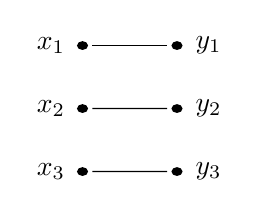
\begin{tikzpicture}[yscale=0.8]
            % Definizione dei nodi x e y con i punti
            \foreach \i in {1,2,3} {
                \node (x\i) at (0, -\i) {$x_\i$};
                \node (y\i) at (2, -\i) {$y_\i$};
                
                % Punti neri
                \fill (0.4, -\i) circle (2pt) node (dotx\i) {};
                \fill (1.6, -\i) circle (2pt) node (doty\i) {};
                
                % Linee di collegamento
                \draw (dotx\i) -- (doty\i);
            }
        \end{tikzpicture}
        
        \vspace{0.3cm}
        \small \textit{Esempio con $M=K=3$}
    \end{minipage}
\end{center}